Prior we begin our discussion it is worth to introduce a few preliminary facts and statements.
Define the iterated rascal number
\begin{definition}
    Iterated rascal number~\cite{gregory2023iterated}
    \begin{align}
        \rascalNumber{n}{k}{i} = \sum_{m=0}^{i} \binom{n-k}{m} \binom{k}{m}
    \end{align}
\end{definition}
First important thing is to notice that iterated rascal number
is a partial case of Vandermonde convolution~\cite{andrews1999special}.
Consider Vandermonde convolution
\begin{equation*}
    \binom{a+b}{r} = \sum_{m=0}^{r} \binom{a}{m} \binom{b}{r-m}
\end{equation*}
Thus,
\begin{equation}
    \rascalNumber{n}{k}{i} = \sum_{m=0}^{i} \binom{n-k}{m} \binom{k}{m} = \sum_{m=0}^{i} \binom{n-k}{m} \binom{k}{k-m}
    \label{eq:rascal-vandermonde-convolution}
\end{equation}
Therefore, iterated rascal number is partial case of Vandermonde convolution with upper summation bound equals to $i$.
Without further hesitation consider our findings.
\begin{proposition}
    Iterated rascal triangle equals to Pascal's triangle up to $i$-th column.
    \begin{equation}
        \rascalNumber{n}{k}{i} = \binom{n}{k}, \quad 0 \leq k \leq i\label{eq:rascal-column-identity}
    \end{equation}
    \begin{proof}
        Proof is given by~\cite{gregory2023iterated}.
    \end{proof}
\end{proposition}
Then binomial identity follows
\begin{align*}
    \rascalNumber{n}{i-k}{i} = \binom{n}{i-k}
\end{align*}
Applying binomial coefficients symmetry principle we obtain
\begin{align*}
    \rascalNumber{n}{n-i+k}{i} = \binom{n}{n-i+k}
\end{align*}
\begin{proposition}
    \label{prop:odd-row-proposition}
    Iterated rascal triangle equals to Pascal's triangle up to $2i+1$-th row
    \begin{align*}
        \rascalNumber{n}{k}{i} = \binom{n}{k}, \quad 0 \leq n \leq 2i+1
    \end{align*}
\end{proposition}
Therefore, for every fixed $i \geq 0$
\begin{equation}
    \rascalNumber{2i+1-n}{k}{i} = \binom{2i+1-n}{k}
    \label{eq:odd-row-identity}
\end{equation}
Equation~\eqref{eq:odd-row-identity} is of interest because in contrast to rascal
column identity~\eqref{eq:rascal-column-identity} it gives relation over $k$ for each $i$,
so that it is true for all cases in $i,k$: $i < k$, $i=k$ and $k >i$.

Taking $t \geq 2i+1$ for every fixed $i \geq 0$
\begin{align*}
    \rascalNumber{t-n}{k}{t-i-1}= \binom{t-n}{k}
\end{align*}
\begin{proof}
    Proof of proposition~\eqref{prop:odd-row-proposition}.
    We have three possible relations between $i,k$: $k<i$, $k=i$, $k > i$.
    So we have to prove that for every $i,k$
    \begin{equation*}
        \sum_{m=0}^{k} \binom{2i+1-n-k}{m} \binom{k}{m} - \sum_{m=0}^{i} \binom{2i+1-n-k}{m} \binom{k}{m} = 0
    \end{equation*}
    For the case $k<i$ proof is given in Jenna Gregory et al.~\cite{gregory2023iterated}.
    For the case $k=i$ proof is trivial.
    Thus, the remaining case is $k>i$ yields that
    \begin{equation*}
        \sum_{m=i+1}^{k} \binom{2i+1-n-k}{m} \binom{k}{m} = 0
    \end{equation*}
    Considering the constraints,
    \begin{equation*}
        \begin{cases}
            n \geq 0 \\
            k \geq i+1 \\
            2i+1-n-k \leq i-n \\
            m \geq i+1
        \end{cases}
    \end{equation*}
    Thus,
    \begin{equation*}
        \sum_{m=i+1}^{k} \binom{2i+1-n-k}{m} \binom{k}{m}
    \end{equation*}
    is indeed equals zero because binomial coefficients $\binom{i-n-s}{i+1+s}$ are zero for each $i, n, s \geq 0$.
    Therefore, the proposition~\eqref{prop:odd-row-proposition} is true.
\end{proof}
Moreover, equation~\eqref{eq:odd-row-identity} gives Vandermonde-like identity
\begin{proposition} (Vandermonde-like identity.)
    \label{prop:vandermonde-like-identity}
    \begin{equation*}
        \binom{2i+1-n}{k} = \sum_{m=0}^{i} \binom{2i+1-n-k}{m} \binom{k}{m}
    \end{equation*}
\end{proposition}
In particular, given $n=0$ proposition~\eqref{prop:vandermonde-like-identity} yields
\begin{equation*}
    \binom{2i+1}{k} = \sum_{m=0}^{i} \binom{2i+1-k}{m} \binom{k}{m}
\end{equation*}

Now, let's smoothly switch our focus to finite differences of binomial coefficients and iterated rascal numbers.
Considering the table of differences $\binom{n}{k}-\rascalNumber{n}{k}{3}$
\begin{figure}[H]
    \centering
    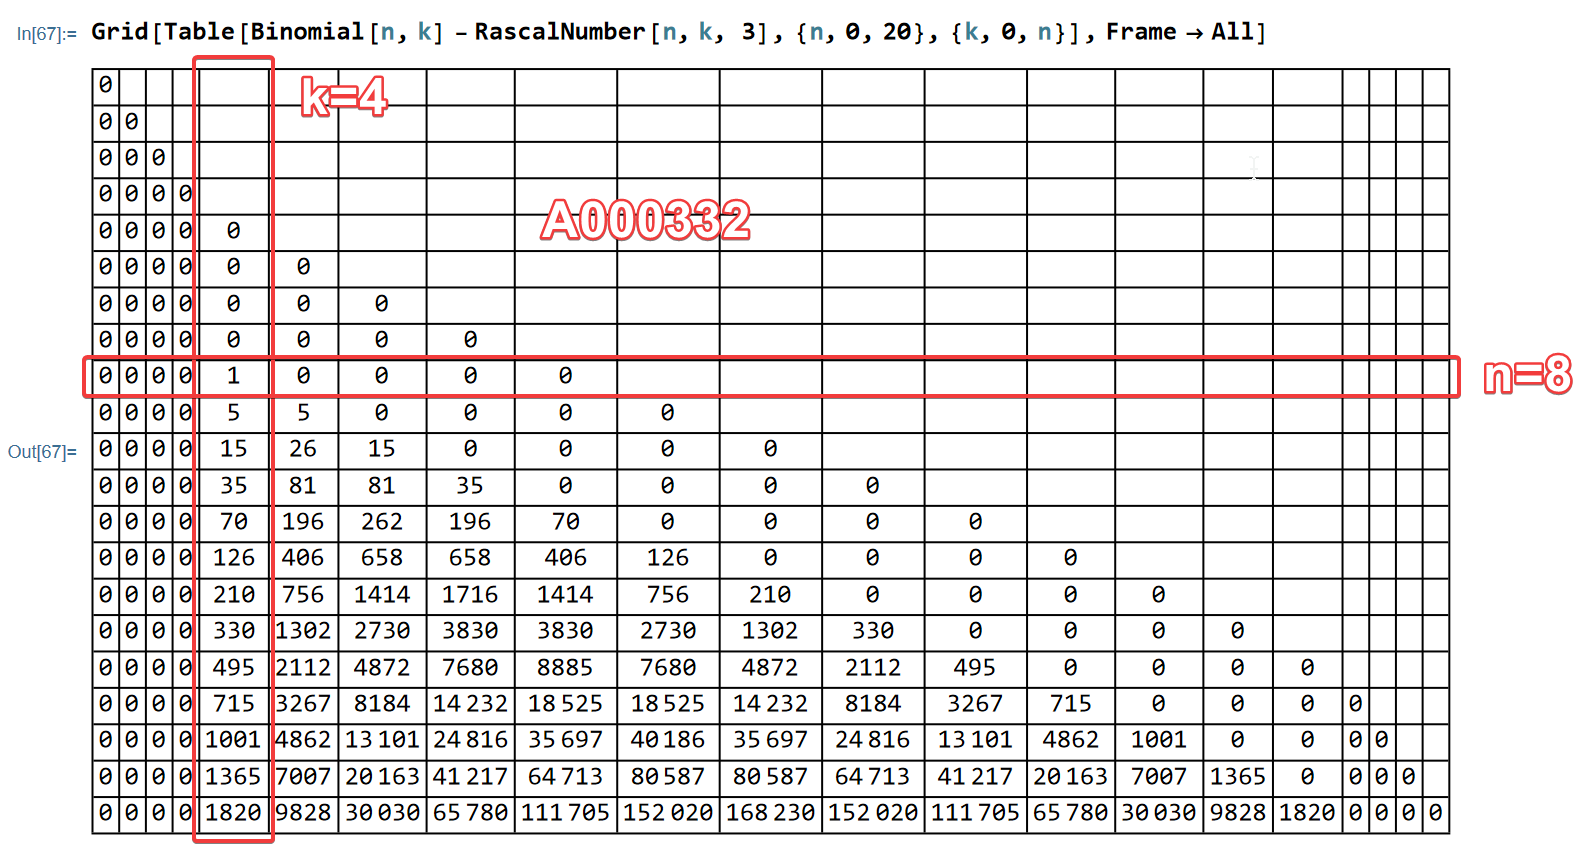
\includegraphics[width=1\textwidth]{img/01_Difference_Binomial_Rascal_i_3_BinomialCoefficients}
    ~\caption{Difference $\binom{n}{k}-\rascalNumber{n}{k}{3}$.
    Highlighted column is $\binom{n}{4}$.
    Sequence \href{https://oeis.org/A000332}{\texttt{A000332}} in the OEIS~\cite{sloane2009binomial}.}
    \label{fig:difference-binomial-rascal-i-3}
\end{figure}
We can spot that having $i=3$ the $k=4$-th column gives binomial coefficient $\binom{n}{4}$.
Indeed, this rule is true for every $i$.
\begin{proposition}
    \label{prop:row-column-difference}
    (Row-column difference.) For every fixed $i\geq0$
    \begin{align*}
        \binom{n+2i}{i} - \rascalNumber{n+2i}{i}{i-1} = \binom{n+i}{i}
    \end{align*}
    \begin{proof}
        We have previously stated that iterated rascal numbers are
        closely related to Vandermonde convolution~\eqref{eq:rascal-vandermonde-convolution}.
        Thus, proposition~\eqref{prop:row-column-difference} can be rewritten as
        \begin{align*}
            \sum_{m=0}^{i} \binom{n+i}{m} \binom{i}{i-m} - \sum_{m=0}^{i-1} \binom{n+i}{m} \binom{i}{m}
        \end{align*}
        Therefore, $\binom{n+2i}{i} - \rascalNumber{n+2i}{i}{i-1} = \binom{n+i}{i}$ is indeed true.
    \end{proof}
\end{proposition}
Proposition~\eqref{prop:row-column-difference} yields to few more identities.
Applying binomial coefficients symmetry
\begin{align*}
    \binom{n+2i}{n+i} - \rascalNumber{n+2i}{n+i}{i-1} &= \binom{n+i}{n}
\end{align*}
Taking $j=n+i$ gives
\begin{align*}
    \binom{j+i}{j} - \rascalNumber{j+i}{j}{i-1} &= \binom{j}{j-i} \\
    \binom{j+i}{i} - \rascalNumber{j+i}{i}{i-1} &= \binom{j}{i}
\end{align*}
Proposition~\eqref{prop:row-column-difference} can be generalized even further, for every fixed $i < k$.
\begin{proposition}
(Binomial coefficient difference iterated rascal number.)
    For every fixed $i < k$
    \label{prop:row-column-difference-general}
    \begin{align*}
        \binom{n}{k} - \rascalNumber{n}{k}{i} &= \sum_{m=i+1}^{k} \binom{n-k}{m} \binom{k}{k-m}
    \end{align*}
    \begin{proof}
        It is true by means of Vandermonde convolution.
    \end{proof}
\end{proposition}
